\documentclass[10pt]{beamer}
\usepackage[ngerman]{babel}
\definecolor{fossaggray}{rgb}{0.1,0.1,0.1}
\definecolor{fossaggreen}{rgb}{0.0,0.7,0.3}
\definecolor{darkgreen}{rgb}{0.0,0.4,0.0}
\usetheme[progressbar=frametitle]{metropolis}
\setbeamercolor{progress bar}{fg=fossaggreen}
\setbeamercolor{frametitle}{bg=fossaggray}
\setbeamercolor{alerted text}{fg=fossaggreen}

\usepackage{appendixnumberbeamer}

\usepackage{booktabs}
\usepackage[scale=2]{ccicons}

\usepackage{pgfplots}
\usepgfplotslibrary{dateplot}

\usepackage{xspace}
\newcommand{\themename}{\textbf{\textsc{metropolis}}\xspace}

\title{Crypto101}
\subtitle{Grundwissen Kryptografie}
% \date{\today}
\date{}
\author{Yannick Bungers}
%\institute{Free and Open Source Software AG}
% \titlegraphic{\hfill\includegraphics[height=1.5cm]{logo.pdf}}

\begin{document}
	
	\maketitle
	
	%\begin{frame}{Table of contents}
	%	\setbeamertemplate{section in toc}[sections numbered]
	%	\tableofcontents%[hideallsubsections]
	%\end{frame}
	
	\section[Ziele von Kryptografie]{Introduction}
	
	\begin{frame}[fragile]{Definition}
		
		Kryptographie bzw. Kryptografie (altgriechisch kryptós, deutsch ‚verborgen‘, ‚geheim‘ und gráphein, deutsch ‚schreiben‘) ist ursprünglich die Wissenschaft der Verschlüsselung von Informationen.
		
		Heute befasst sie sich auch allgemein mit dem Thema Informationssicherheit, also der Konzeption, Definition und Konstruktion von Informationssystemen, die widerstandsfähig gegen Manipulation und unbefugtes Lesen sind.\\
		\vspace{0.35cm} 
		\textit{Wikipedia: Kryptografie}
		%\begin{verbatim}    \documentclass{beamer}
			%\usetheme{metropolis}\end{verbatim}
		
		%Note, that you have to have Mozilla's \emph{Fira Sans} font and XeTeX
		%installed to enjoy this wonderful typography.
	\end{frame}
	\begin{frame}[fragile]{Sicherheitsziele}
		\begin{itemize}
			\item \alert{Vertraulichkeit/Zugriffsschutz}: keine Informationen über den Inhalt
			\vspace{0.5cm}
			\item \alert{Integrität/Änderungsschutz}: vollständig und unverändert
			\vspace{0.5cm}
			\item \alert{Authentizität/Fälschungsschutz}: Absender identifizierbar
			\vspace{0.5cm}
			\item \alert{Verbindlichkeit/Nichtabstreitbarkeit}: Urheberschaft ist nachweisbar
		\end{itemize}
		
	\end{frame}
	
	\section{Grundbegriffe}
	
	\begin{frame}{symmetrische Verschlüsselung}
		\alert{Schlüssel} \texttt{k}\\
		\alert{Eingabe} \texttt{t}\\
		\alert{Ciphertext} \texttt{c}\\
		\vspace{0.5cm}
		Für Ver- und Entschlüsselung wird der gleiche Schlüssel verwendet.\\
		\texttt{Enc(t, k) = c}\\
		\texttt{Dec(c, k) = t}\\
		Ziel: Vertraulickeit, (Integrität), (Authenzität)
	\end{frame}
	
	\begin{frame}{Asymmetrische Verschlüsselung}
		\alert{Privater Schlüssel} \texttt{privk}\\
		\alert{Öffentlicher Schlüssel} \texttt{pubk}\\
		\alert{Eingabe} \texttt{t}\\
		\alert{Ciphertext} \texttt{c}\\
		\vspace{0.5cm}
		Für Ver- und Entschlüsselung werden andere aber abhängige Schlüssel verwendet (Schlüsselpaar).
		Der \emph{private} Schlüssel darf nicht aus dem \emph{öffentlichen} Schlüssel ableitbar sein.\\
		\texttt{Enc(t, pubk) = c}\\
		\texttt{Dec(c, privk) = t}\\
		\alert{Ziel}: Vertraulickeit, (Integrität)\\
	\end{frame}

	\begin{frame}{Signaturen}
		\alert{Privater Schlüssel} \texttt{privk}\\
		\alert{Öffentlicher Schlüssel} \texttt{pubk}\\
		\alert{Eingabe} \texttt{t}\\
		\alert{Signatur} \texttt{s}\\
		\vspace{0.5cm}
		Die Signatur wird mit dem privaten Schlüssel erzeugt und mit dem öffentlichen Schlüssel verifiziert.\\
		\texttt{Enc(t, privk) = s}\\
		\texttt{Dec(s, pubk) = t}\\
		\alert{Ziel}: (Integrität), Authenzität, Nichtabstreitbarkeit\\
	\end{frame}


	\begin{frame}{Diffie-Hellman-Key-Exchange}
		Der Schlüsselaustausch ist ein sehr zentrales Element der Sicherheit von Kryptografie. Mit Hilfe des Diffie-Hellman-Key-Exchange-Verfahrens ist es möglich einen symmetrischen Schlüssel über eine unsichere Verbindung zu etablieren ohne das ein dritter aus den gesendet Nachrichten den Schlüssel ableiten kann.
	\end{frame}
	\begin{frame}{symmetrische vs. Asymmetrische Verschlüsselung}
		\begin{alertblock}{symmetrische Verschlüsselung}
			\begin{itemize}
				\item schnell und resourcenschonend
				\item nicht vollständig gebrochen durch Quantencomputer
			\end{itemize}
		\end{alertblock}
		\begin{alertblock}{Asymmetrische Verschlüsselung}
			\begin{itemize}
				\item ein Key pro Partei statt ein Key pro Verbindung
				\item jeder kann Verschlüsseln
			\end{itemize}
		\end{alertblock}
	\end{frame}

	\begin{frame}{Hashfunktionen}
		\center{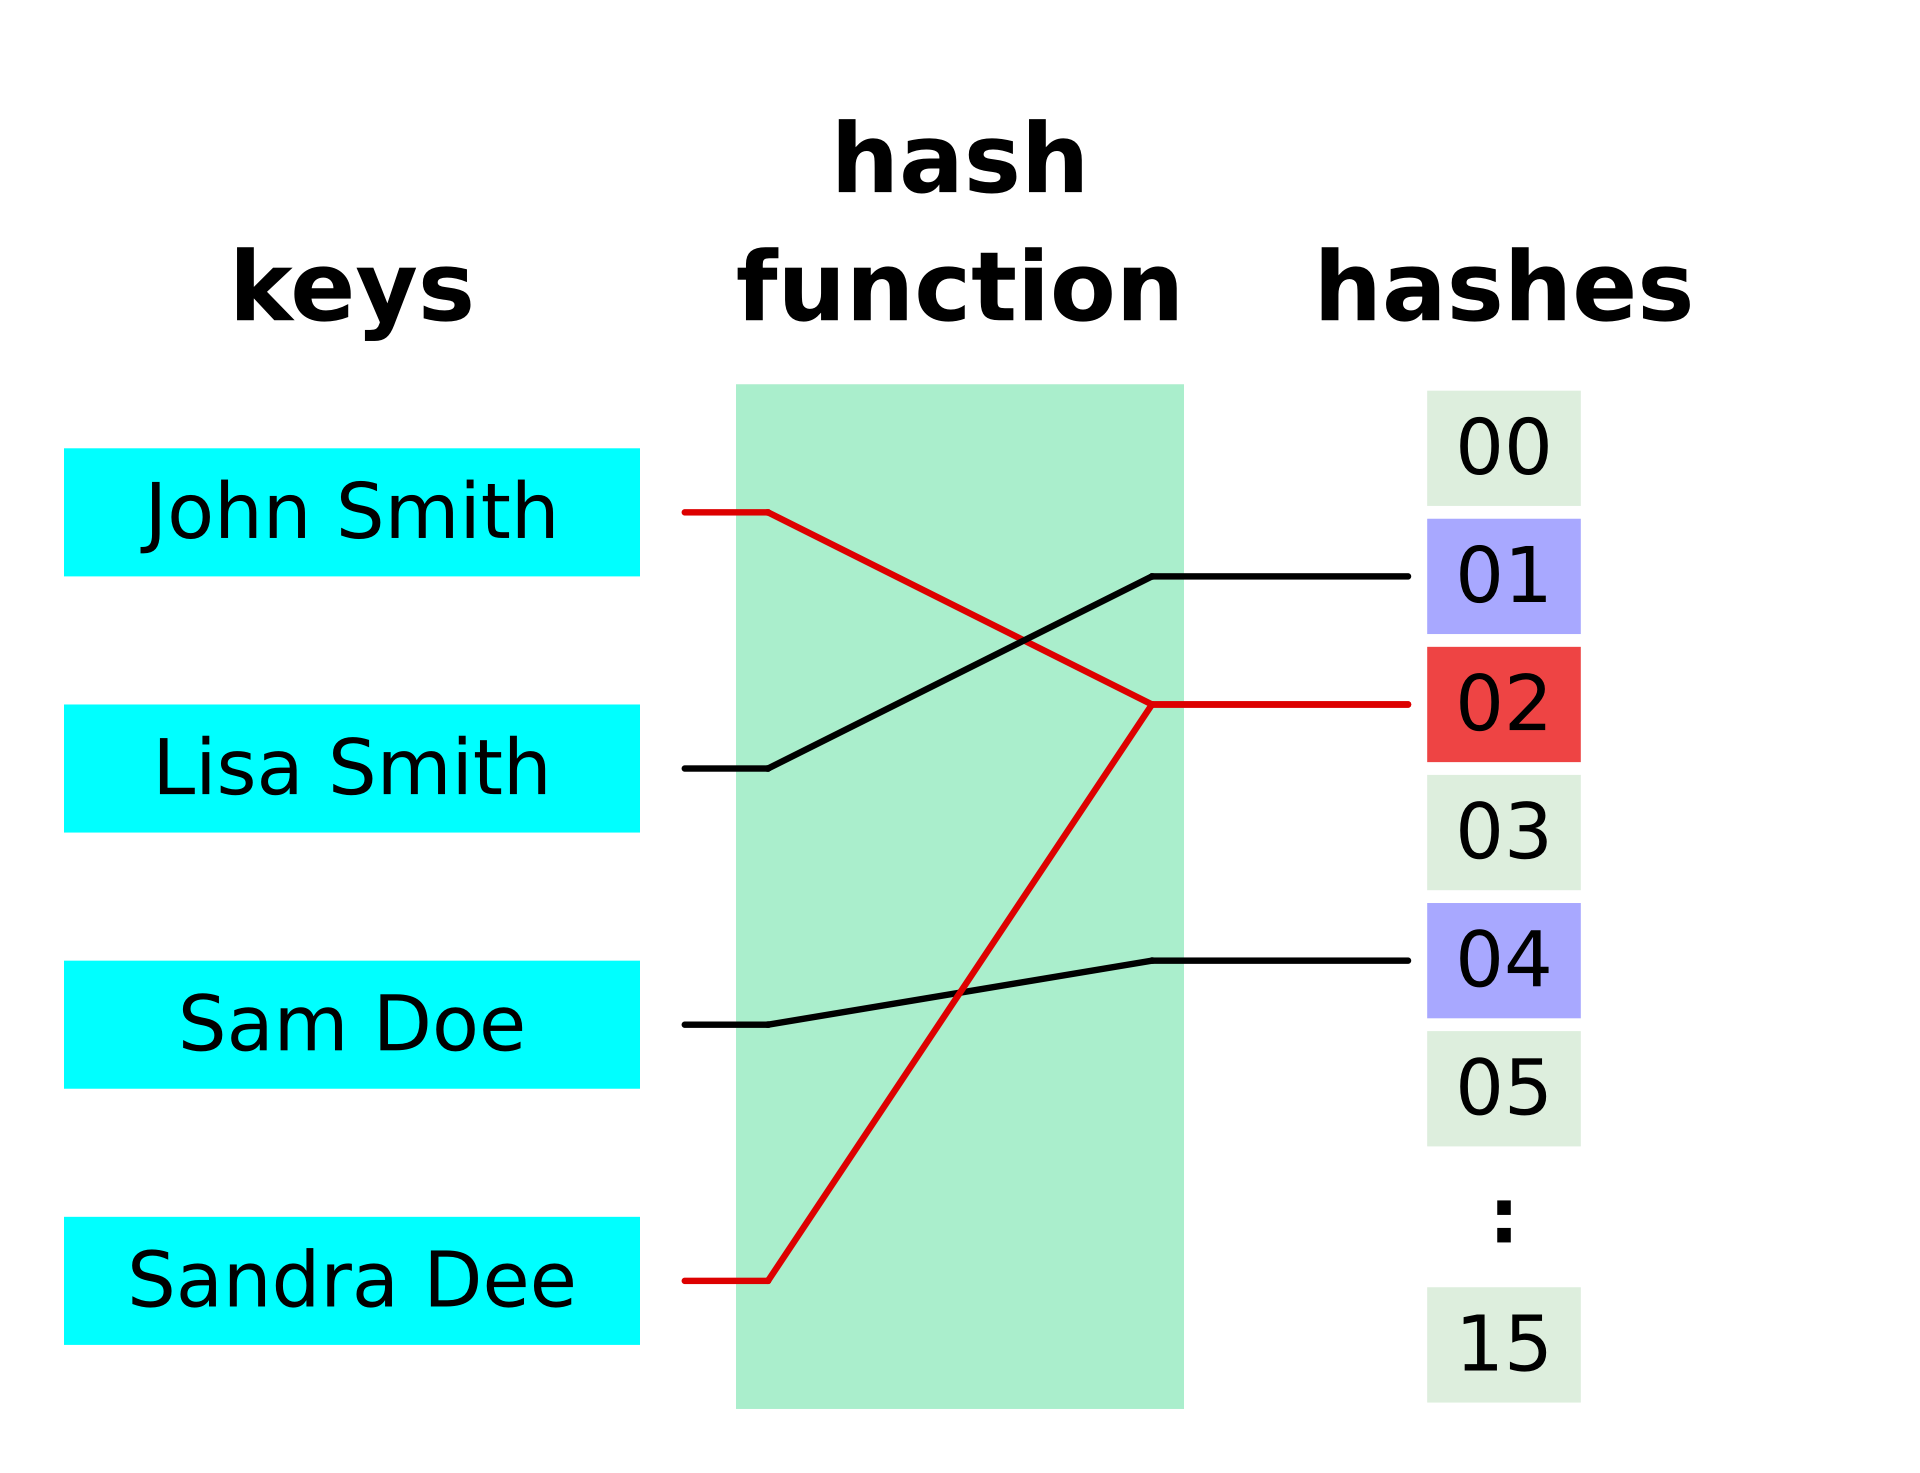
\includegraphics[scale=0.2]{hashtable.png}}
	\end{frame}

	\begin{frame}{Kryptografische Hashfunktionen}
		\begin{alertblock}{Voraussetzungen für gute Hashfunktionen}
			\begin{itemize}
				\item Geringe Wahrscheinlichkeit für Kollisionen
				\item Keine unmöglichen Werte
				\item Effizienz
			\end{itemize}
		\end{alertblock}
		\begin{alertblock}{Kryptografische Voraussetzungen}
			\begin{itemize}
				\item \textbf{Chaos oder Lawineneffekt}\\
				Ähnliche Eingabe, völlig verschiedene Hashwerte
				\item \textbf{Konfusion}\\
				Keine Möglichkeit des Rückschlusses von Hashwert auf die Eingabe
				\item \textbf{Unumkehrbarkeit}\\
				Keine Möglichkeit aus Hash eine passende Eingabe zu berechnen
			\end{itemize}
			
		\end{alertblock}
	\end{frame}

	\begin{frame}{Zufallszahlen}
		\begin{itemize}
			\item Sehr relevanter Teil von Kryptografie
			\item Schlüssel werden häufig aus Zufallszahlen generiert
			\item Ein sehr relevanter Teil von Kryptografie ist, dass der Suchraum für Brute Force angriffe groß ist, bei schlechten Zufallszahlen wird dieser bereich häufig sehr viel kleiner.
		\end{itemize}
	\end{frame}
	
	\section{Praxis}
	
	\begin{frame}{Verknüpfung von Grundlagen}
		Häufig werden diverse Techniken verbunden:
		\begin{itemize}
			\item erst hashen dann den Hash signieren
			\item Austausch eines Session Keys mit asymmetrischer Kryptografie um dann mit symmetrischer Kryptograpie Daten zu übertragen.
			\item Signatur und Verschlüsselung um alle angesprochenen Sicherheitsziele zu gewährleisten
		\end{itemize}
	\end{frame}

	\begin{frame}{symmetrische Verschlüsselung in der Praxis}
		\begin{alertblock}{Unsichere bzw. nicht empfohlene Beispiele}
			\begin{itemize}
				\color{red}
				\item DES, Triple-DES
				\item RC2, RC4, RC5
			\end{itemize}
		\end{alertblock}
		\begin{alertblock}{Sichere Beispiele}
			\begin{itemize}
				\color{darkgreen}
				\item AES (128 [nicht für postquanten], 192, 256)
				\item blowfish
				\item twofish
				\item RC6
				\item Serpent
			\end{itemize}
		\end{alertblock}
	\end{frame}
	
	\begin{frame}{Hashverfahren in der Praxis}
		\begin{alertblock}{Unsichere Beispiele für Kryptografie}
			\begin{itemize}
				\color{red}
				\item MD2, MD4, MD5
				\item SHA0, SHA1
				\item RIPEMD
			\end{itemize}
		\end{alertblock}
		\begin{alertblock}{Sichere Beispiele}
			\begin{itemize}
				\color{darkgreen}
				\item SHA2 (SHA256, SHA384, SHA512) [Length extension possible]
				\item SHA3
				\item BLAKE2s, BLAKE2b, BLAKE3
			\end{itemize}
		\end{alertblock}
		\begin{alertblock}{Für Passwörter}
			\vspace{0.1cm}
			Es ist zusätzlich ein Salt nötig um Rainbow-Tables nutzlos zu machen.
			\vspace{-0.2cm}
			
		\begin{itemize}
			\color{darkgreen}
			\item bcrypt
			\item argon2
		\end{itemize}
	\end{alertblock}
	\end{frame}
	
	\begin{frame}{Asymmetrische Kryptografie in der Praxis}
		Für viele Anwendungen wird nur eine Signatur benötigt, da nur sichergestellt werden muss, dass man mit dem richtigen gegenüber kommuniziert, da das Diffie-Hellman-Verfahren einen Key-Austausch über eine unsichere Verbindung ermöglicht. Dies ermöglicht außerdem, dass perfect forward secrecy möglich ist, mit anderen Worten, dass auch bei bekannt werden des privaten Schlüssels nicht alle alten Nachrichten entschlüsselt werden können.
		
		\begin{alertblock}{Beispiele}
			\begin{itemize}
				\item SSH
				\item modernes TLS
			\end{itemize}
		\end{alertblock}
		
		Für z.B. E-Mail-Verschlüsselung hingegen, muss eine asymmetrische Verschlüsselung verwendet werden, da kein Kanal besteht.
	\end{frame}

	\begin{frame}{TLS}
		\begin{itemize}
			\item enstanden aus SSL
			\item Protokoll zur Verschlüsselung von Daten eine Netzwerkverbindung
			\item Zusammenstellung von möglichen Algorithmen
			\item Zertifikate werden in einer Public Key Infrastructure ausgegeben
		\end{itemize}
		\begin{alertblock}{Versionen}
			\begin{itemize}
				\color{red}
				\item 1.0 (SSL 3.0)
				\item 1.1
				\color{darkgreen}
				\item 1.2
				\item 1.3
			\end{itemize}
		\end{alertblock}
	\end{frame}
\end{document}